\section{Design Entry Using VHDL Code}


\noindent
As a design example, we will use the two-way light controller circuit illustrated in 
Figure~\ref{fig:11}. This circuit can be used to control a single light from either of the
two switches $x_1$ and $x_2$, where a closed switch corresponds to the logic value 1.
The truth table for the circuit is also given in the figure. Note that
this is just the Exclusive-OR function of the inputs $x_1$ and $x_2$,
but we will specify it using the gates shown.

\begin{figure}[H]
   \begin{center}
      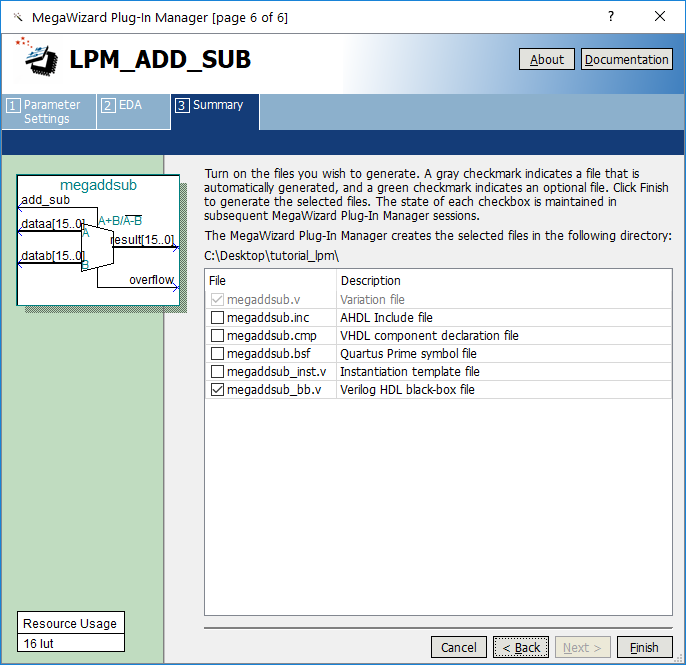
\includegraphics[scale=1]{figures/figure11.png}
   \caption{The light controller circuit.} 
	 \label{fig:11}
	 \end{center}
\end{figure}

The required circuit is described by the VHDL code in Figure~\ref{fig:12}.
Note that the VHDL entity is called {\it light} to match the name given in 
Figure~\ref{fig:4}, which was specified when the project was created.
This code can be typed into a file by using any text editor
that stores ASCII files, or by using the Quartus Prime text editing facilities.
While the file can be given any name, it is a common designers' practice to
use the same name as the name of the top-level VHDL entity.
The file name must include the extension $vhd$, which indicates a VHDL
file. So, we will use the name {\it light.vhd}.

\lstset{language=VHDL} 
\begin{figure}[H]
\begin{center}
\begin{minipage}[h]{12.5 cm}
\begin{lstlisting}
LIBRARY ieee ;
USE ieee.std_logic_1164.all ;

ENTITY light IS
	PORT(x1, x2	: IN	STD_LOGIC ;
		 f		: OUT	STD_LOGIC);
END light ;

ARCHITECTURE LogicFunction OF light IS
BEGIN
	f <=	(x1 AND NOT x2) OR (NOT x1 AND x2) ;
END LogicFunction ;
\end{lstlisting}
\end{minipage}
\end{center}
	\caption{VHDL code for the circuit in Figure \ref{fig:11}.}

	\label{fig:12}
\end{figure}

\subsection{Using the Quartus Prime Text Editor}

\noindent 
This section shows how to use the Quartus Prime Text Editor.
You can skip this section if you prefer to use some other text editor
to create the VHDL source code file, which we will name {\it light.vhd}. 

Select {\sf File $>$ New} to get the window in Figure~\ref{fig:13}, 
choose {\sf VHDL File}, and click {\sf OK}. 
This command opens the Text Editor window.  The first step is to specify a name
for the file that will be created. Select {\sf File $>$ Save As}
to open the pop-up box depicted in Figure~\ref{fig:14}. 
In the box labeled {\sf Save as type} choose {\sf VHDL File}.
The name of the file in the box labeled {\sf File name} should be {\it light}.
Put a check-mark in the box {\sf Add file to current project}.
Click {\sf Save}, which puts the file into the directory
{\it introtutorial} and leads to the Text Editor window shown
in Figure~\ref{fig:15}. 
Enter the VHDL code in Figure~\ref{fig:12}
into the Text Editor and save the file by typing {\sf File $>$ Save}, or by typing 
the shortcut {\sf Ctrl-s}.

Most of the commands available in the Text Editor are self-explanatory. 
Text is entered at the {\it insertion point}, which is indicated by a thin
vertical line. The insertion point can be moved either by using the
keyboard arrow keys or by using the mouse. Two features of 
the Text Editor are especially convenient for typing VHDL
code. First, the editor can display different types of VHDL
statements in different colors, which is the default choice. 
Second, the editor can automatically
indent the text on a new line so that it matches the previous line. 
Such options can be controlled by the settings 
in {\sf Tools $>$ Options $>$ Text Editor}.

\begin{figure}[H]
   \begin{center}
      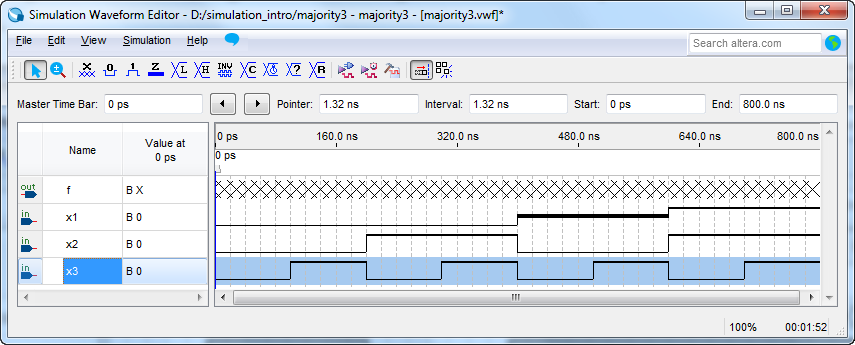
\includegraphics[scale=0.65]{figures/figure13.png}
   \caption{Choose to prepare a VHDL file.} 
	 \label{fig:13}
	 \end{center}
\end{figure}

\begin{figure}[H]
   \begin{center}
      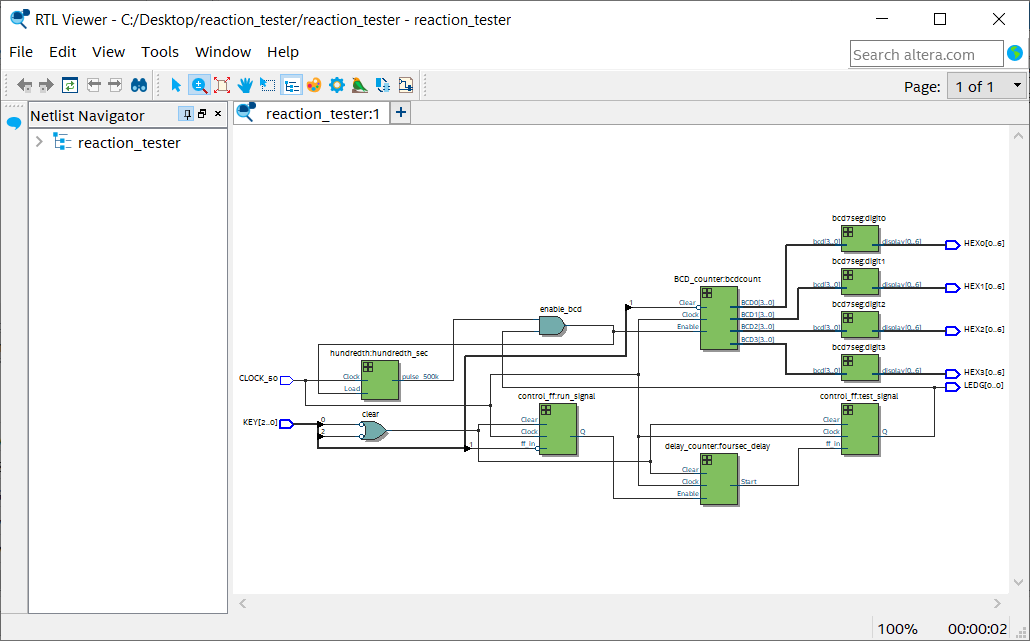
\includegraphics[scale=0.6]{figures/figure14.png}
   \caption{Name the file.} 
	 \label{fig:14}
	 \end{center}
\end{figure}

\begin{figure}[H]
   \begin{center}
      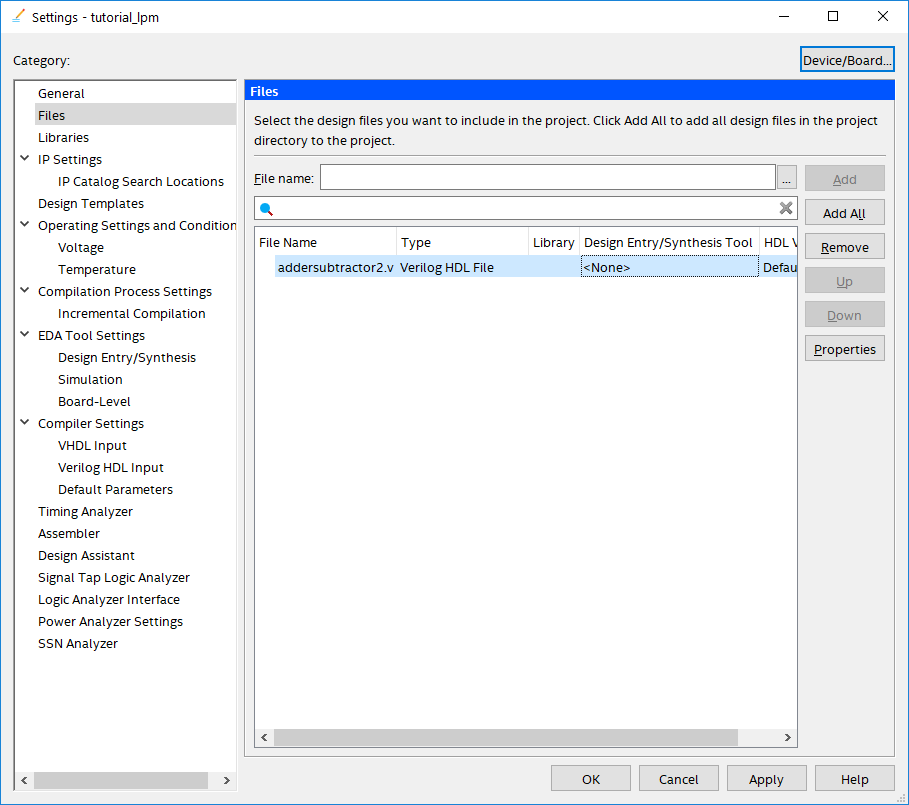
\includegraphics[scale=0.45]{figures/figure15.png}
   \caption{Text Editor window.} 
	 \label{fig:15}
	 \end{center}
\end{figure}

\subsubsection{Using VHDL Templates}

The syntax of VHDL code is sometimes difficult for a
designer to remember. To help with this issue, the Text Editor
provides a collection of {\it VHDL templates}. The templates provide
examples of various types of VHDL statements, such as an {\bf ENTITY}
declaration, a {\bf CASE} statement, and assignment statements. 
It is worthwhile to browse through the templates
by selecting {\sf Edit $>$ Insert Template $>$ VHDL} to become 
familiar with this resource.

\subsection{Adding Design Files to a Project}

As we indicated when discussing Figure~\ref{fig:6}, you can tell the Quartus Prime software
which design files it should use as part of the current project.
To see the list of files already included in the {\it light} project,
select {\sf Assignments $>$ Settings}, which leads to the window in Figure~\ref{fig:16}.
As indicated on the left side of the figure, click on the item {\sf Files}.
An alternative way of making this selection is to choose
{\sf Project $>$ Add/Remove Files in Project}.

If you used the Quartus Prime Text Editor to create the file and checked
the box labeled {\sf Add file to current project},
as described in Section 5.1, then the {\it light.vhd}
file is already a part of the project and will be listed in
the window in Figure~\ref{fig:16}.
Otherwise, the file must be added to the project. 
So, if you did not use the Quartus Prime Text Editor, then place a copy of the 
file {\it light.vhd}, which you created using some other text editor, into 
the directory {\it introtutorial}.
To add this file to the project, click on the {\sf ...} button next to the 
box labeled {\sf File name} in
Figure~\ref{fig:16} to get the pop-up window in Figure~\ref{fig:17}.
Select the {\it light.vhd} file and click {\sf Open}.
The selected file is now indicated in the {\sf File name} box in Figure~\ref{fig:16}. 
Click {\sf Add} then {\sf OK} to include the {\it light.vhd} file in the project.
We should mention that in many cases the Quartus Prime software is able to 
automatically find the right files to use for each entity 
referenced in VHDL code, even if the file has not been 
explicitly added to the project. However, for complex projects that
involve many files it is a good design practice to specifically
add the needed files to the project, as described above.

\begin{figure}[H]
   \begin{center}
      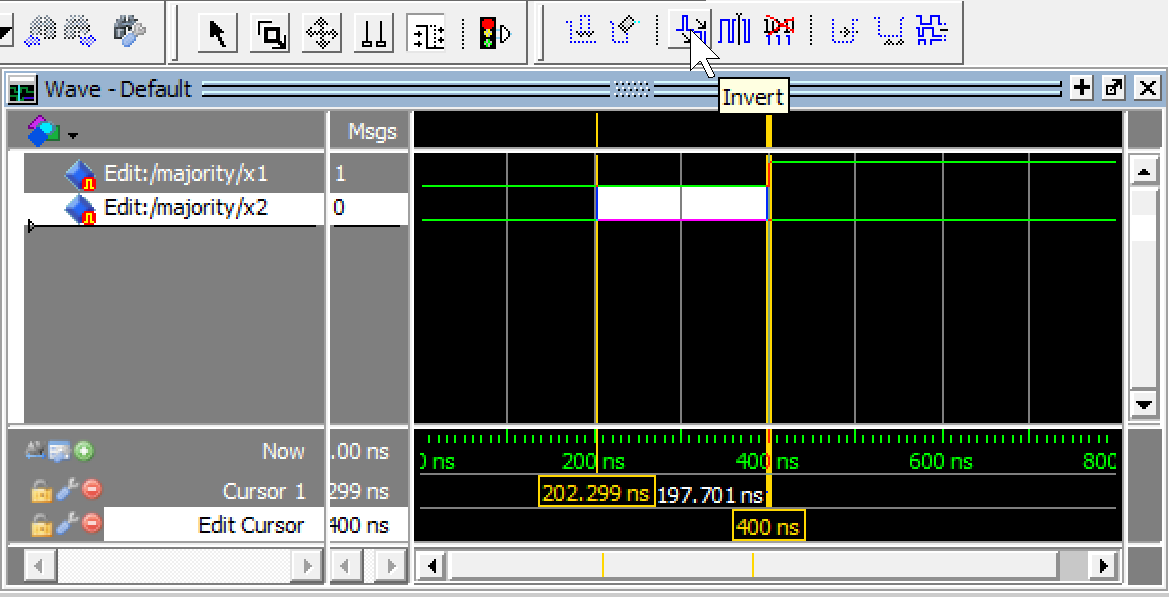
\includegraphics[scale=0.65]{figures/figure16.png}
   \caption{Settings window.} 
	 \label{fig:16}
	 \end{center}
\end{figure}

\begin{figure}[H]
   \begin{center}
      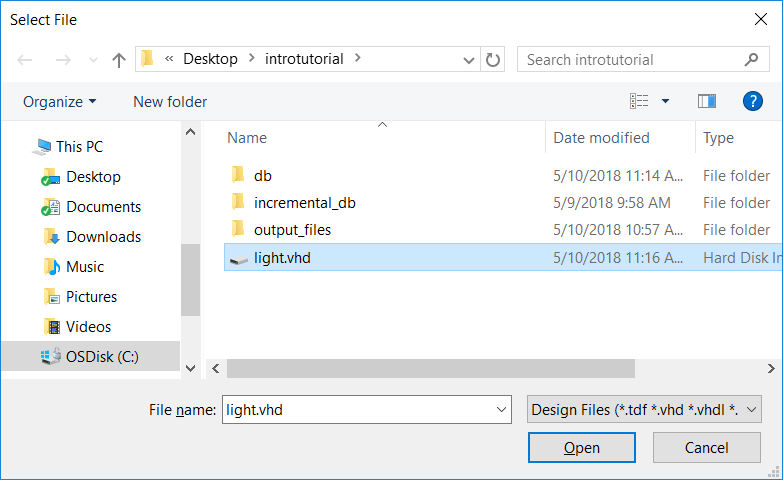
\includegraphics[scale=0.65]{figures/figure17.png}
   \caption{Select the file.} 
	 \label{fig:17}
	 \end{center}
\end{figure}
